
\documentclass[fleqn,addpoints]{exam}
\usepackage{amsmath}
\usepackage{graphicx}
\usepackage{float}
\usepackage{caption}
\usepackage{polynom}

\printanswers

\ifprintanswers
\usepackage{2in1, lscape}
\fi

\title{Math 115 Chapter Two Exam}
\date{February 1, 2011}

\author{}

\begin{document}

\maketitle

\ifprintanswers
\else
\vspace{0.2in}
\makebox[\textwidth]{Name:\enspace\hrulefill}
\vspace{0.2in}

\begin{center}
\gradetable[h][pages]
% \bonusgradetable[h][pages]
\end{center}

\fi

\section{Polynomial Division} 

\begin{questions}

\question[5]
Use synthetic division to divide: $\dfrac{x^4-4x^3-2x^2+12x+11}{x-3}$

\begin{solution}[5 cm]
\[
  \polyhornerscheme[x=3]{x^4-4x^3-2x^2+12x+11}
\]

\[
  \dfrac{x^4-4x^3-2x^2+12x+11}{x-3} = x^3-x^2-5x-3 + \frac{2}{x-3}
\]
\end{solution}
 
\question[5]
$f(x) = 3x^4 -11x^3 - 20x + 5$.  Use synthetic division to find $f(4)$

\begin{solution}[6 cm]
\[
  \polyhornerscheme[x=4]{3x^4 -11x^3 - 20x + 5}
\]

so $f(4) = -11$

\end{solution}

\question[5]
Use synthetic division to determine if $\left(x-\dfrac{2}{3} \right)$ is a factor of $f(x) = 6x^3-x^2-5x+2$.

\begin{solution}[6 cm]
\[
  \polyhornerscheme[x=\frac{2}{3}]{6x^3-x^2-5x+2}
\]

The remainder is zero so $\left(x-\dfrac{2}{3} \right)$ is a factor.

\end{solution}
 
\section{Zeros and Factoring}

\question
$f(x) = 2x^4 + 3x^3 + x^2 - 17$.  Use {\em Descarte's Rule of Signs} to determine how many zeros $f$ may have.

\begin{parts}
\part[2] How many positive zeros does $f$ have?

\begin{solution}[2 cm]
$f(x)$ has one change of sign so there is 1 positive zero.
\end{solution}

\part[3] How many negative zeros might $f$ have?

\begin{solution}[3 cm]
\[
  f(-x) = 2x^4 - 3x^3 + x^2 - 17
\]

$f(-x)$ has 3 changes of sign, so there are 1 or 3 negative solutions.

\end{solution}
\end{parts}

\question[5]
$f(x) = 2x^3 + 7x^2 - 13x + 12$.  Use the {\em Rational Zero Test} to list all the possible rational zeros of $f$.

\begin{solution}[3 cm]
  After removing duplicates, the possibilities are:
\[
  x = \left \{ \pm 1, \pm 2, \pm 3, \pm 4, \pm 6, \pm 12, \pm \dfrac{1}{2}, \pm \dfrac{3}{2} \right \}
\]

\end{solution}

\question[10]
Factor completely and find all the zeros of $f(x) = x^3 - 2x^2 - 13x - 10$

\begin{solution}[8 cm]
\[ 
  \polyhornerscheme[x=-1]{x^3 - 2x^2 - 13x - 10}
\]

\begin{align*}
  f(x) &= (x+1)(x^2-3x+10) \\
       &= (x+1)(x+2)(x-5)
\end{align*}

The zeros are: $x = \{-2, -1, 5\}$

\end{solution}

\question[10]
Factor completely to find all the zeros of $f(x) = 2x^3 + x^2 - 8x - 4$

\begin{solution}[8 cm]
\[ 
  \polyhornerscheme[x=-\frac{1}{2}]{2x^3 + x^2 - 8x - 4}
\]

\begin{align*}
  f(x) &= \left( x+\frac{1}{2} \right) (2x^2-8) \\
       &= 2 \left( x+\frac{1}{2} \right) (x^2-4) \\
       &= (2x+1)(x+2)(x-2) \\
\end{align*}

The zeros are: $x = \left \{ -\dfrac{1}{2}, -2, 2 \right \}$

\end{solution}

\ifprintanswers
\else
\pagebreak 
\fi

\question[10]
Find a polynomial with real coefficients with zeros at $x = \{ -3, 2, 2i \}$.  Of course your polynomial will also have at
least one more zero, since there is no polynomial with real coefficients and just these three zeros.

\begin{solution}[8 cm]

Since $2i$ is a zero, its conjugate, $-2i$ will also be a zero.

\begin{align*}
  f(x) &= (x+3)(x-2)(x+2i)(x-2i) \\ 
    &= (x^2+x-6)(x^2+4) \\ 
    &= x^4 + x^3 - 2x^2 + 4x - 24 \\ 
\end{align*}

\end{solution}

\ifprintanswers
\pagebreak
\fi

\question[10]
$f(x) = 3x^4 + 5x^3 + x^2 + 5x - 2$.  $x = i$ is one zero.  Find the others.

\begin{solution}[7 cm]
Since $i$ is a zero, its conjugate, $-i$ will also be a zero.  $(x-i)$ and $(x+i)$ are both factors, so $(x+i)(x-i) =
x^2+1$ is also a factor.

\[ 
  \polylongdiv{3x^4 + 5x^3 + x^2 + 5x - 2}{x^2+1}
\]

\begin{align*}
  f(x) &= (x+i)(x-i)(3x^2+5x-2) \\
  &= (x+i)(x-i)(3x-1)(x+2) \\
\end{align*}

The zeros are: $x = \left \{ i, -i, \dfrac{1}{3}, -2 \right \}$

\end{solution}

\pagebreak

\section{Graphing}
For questions \ref{graph:1}-\ref{graph:3}, find all intercepts and asymptotes, check for
symmetry, and plot the graph.

\question[10]
\label{graph:1}
\[
  f(x) = x^5 - 4x^4 + 4x^3
\]

\begin{solution}[6 cm]
\[
  f(x) = x^5 - 4x^4 + 4x^3 = x^3(x^2 - 4x + 4) = x^3(x-2)^2
\]

\begin{itemize}
  \item the graph will look like the graph of $y=x^5$ for very large or very small values of x.
  \item there is a zero of multiplicity 3 at $x=0$ and a zero of multiplicity 2 at $x=2$.  This means that the graph
    will cross the x axis at $x=0$ and touch but not cross at $x=2$.
  \item there isn't any symmetry
  \item $f(0) = 0$, so the y intercept is at $y=0$
  \item there aren't any asymptotes since the function isn't a fraction
\end{itemize}

\end{solution}

\ifprintanswers
\begin{figure}[H]
  \centering
  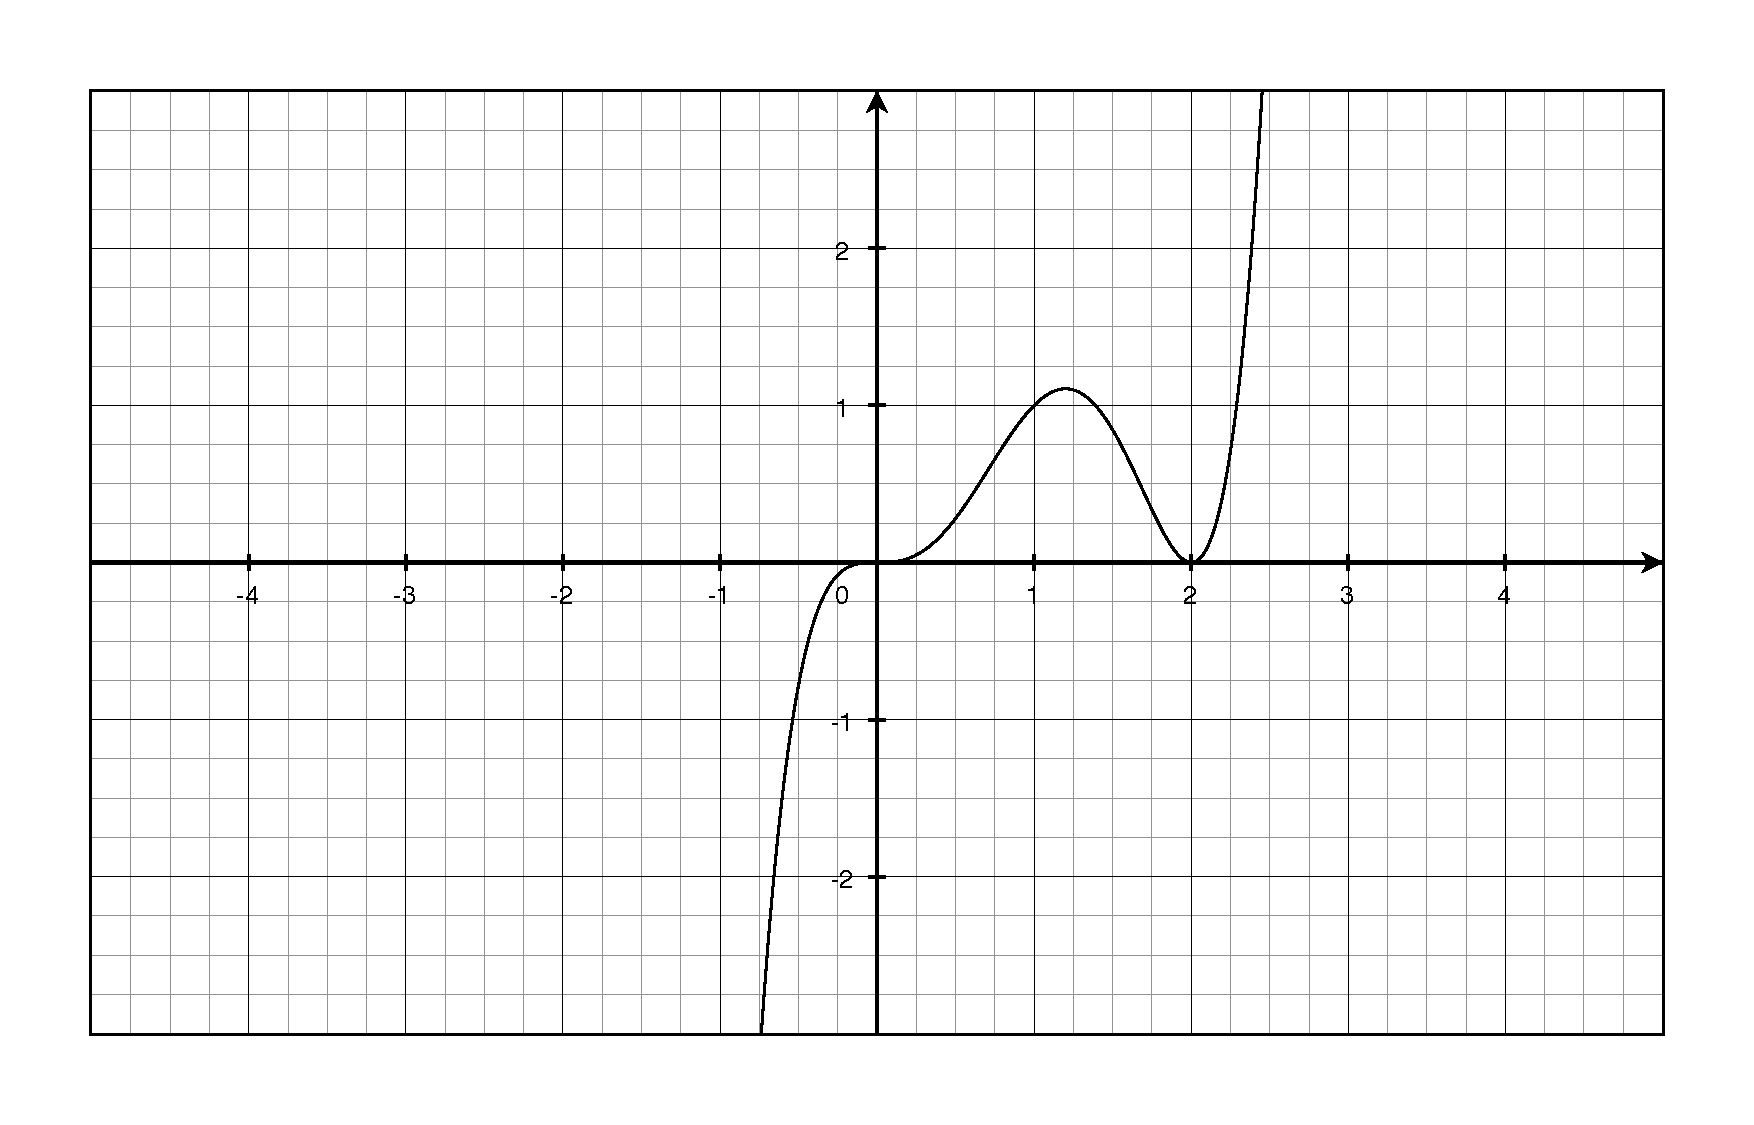
\includegraphics[scale=0.4]{graph_1_solution.eps}
  \caption*{Question \ref{graph:1}}
\end{figure}
\else
\begin{figure}[H]
  \centering
  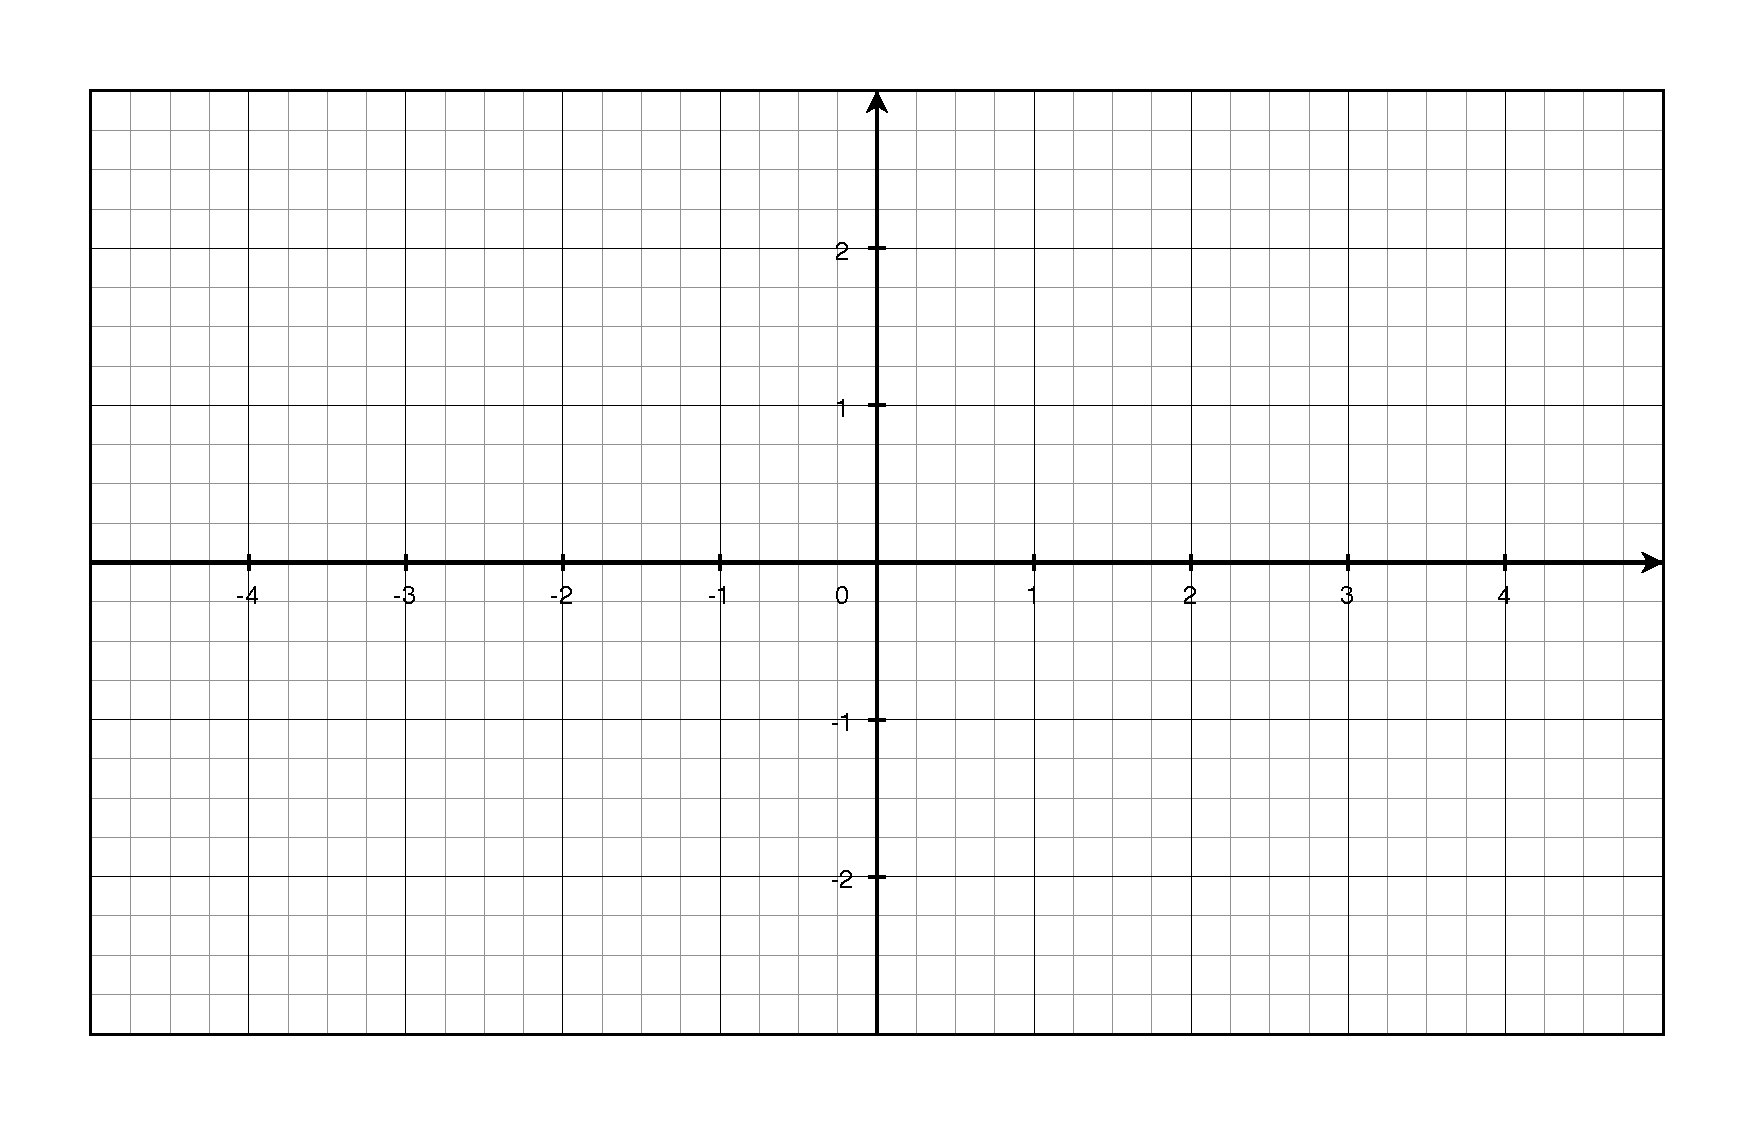
\includegraphics[scale=0.6]{graph_1_blank.eps}
  \caption*{Question \ref{graph:1}}
\end{figure}
\fi

\ifprintanswers
\else
\pagebreak
\fi

\question[10]
\label{graph:2}

\[
  f(x) = \frac{x^2}{2x^2-8}
\]

\begin{solution}[6 cm]
\[
  f(x) = \frac{x^2}{2x^2-8} = \frac{x^2}{2(x^2-4)} = \frac{x^2}{2(x+2)(x-2)}
\]

\begin{itemize}
  \item there is a zero at $x=0$
  \item $f(x) = f(-x)$ so there is y axis symmetry
  \item $f(0) = 0$, so the y intercept is at $y=0$
  \item the degree of the numerator is the same as the degree of the denominator, so there is a horizontal asymptote at
    $y = \dfrac{1}{2}$
  \item there are vertical asymptotes at $x=\pm 2$
\end{itemize}

\end{solution}

\ifprintanswers
\begin{figure}[H]
  \centering
  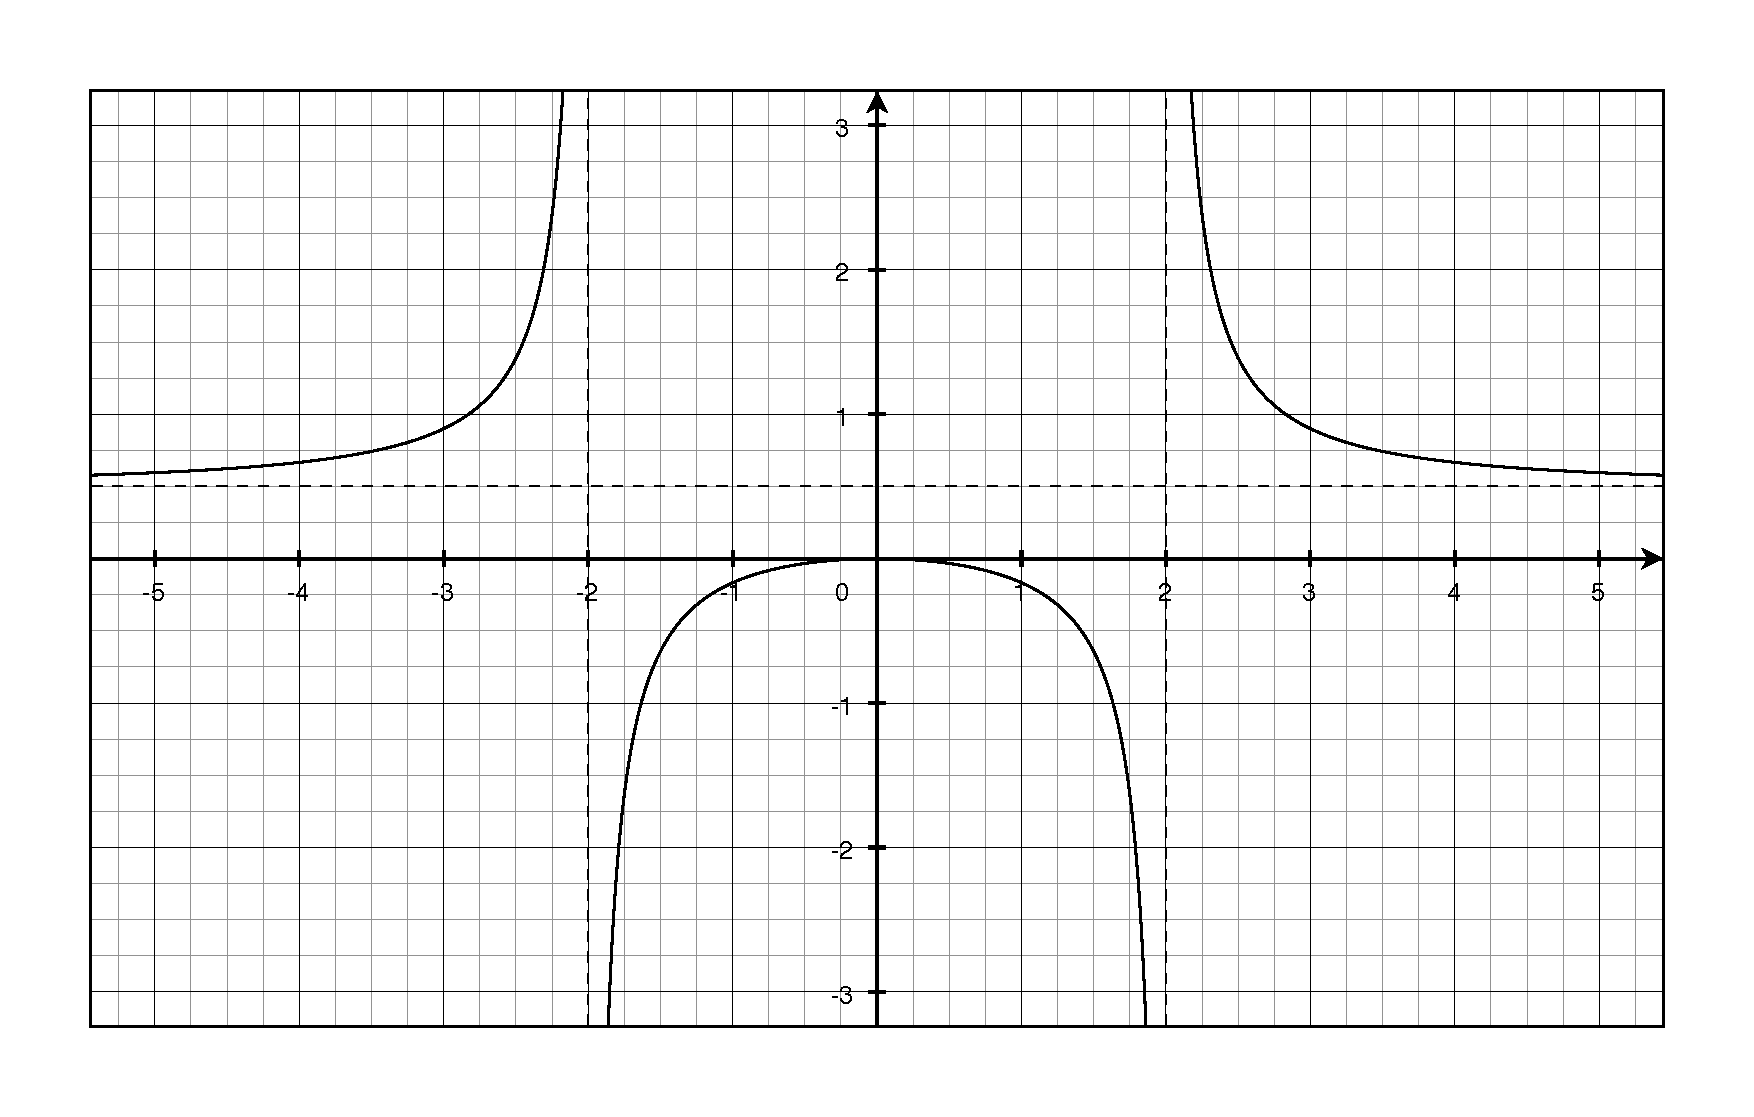
\includegraphics[scale=0.4]{graph_2_solution.eps}
  \caption*{Question \ref{graph:2}}
\end{figure}
\else
\begin{figure}[H]
  \centering
  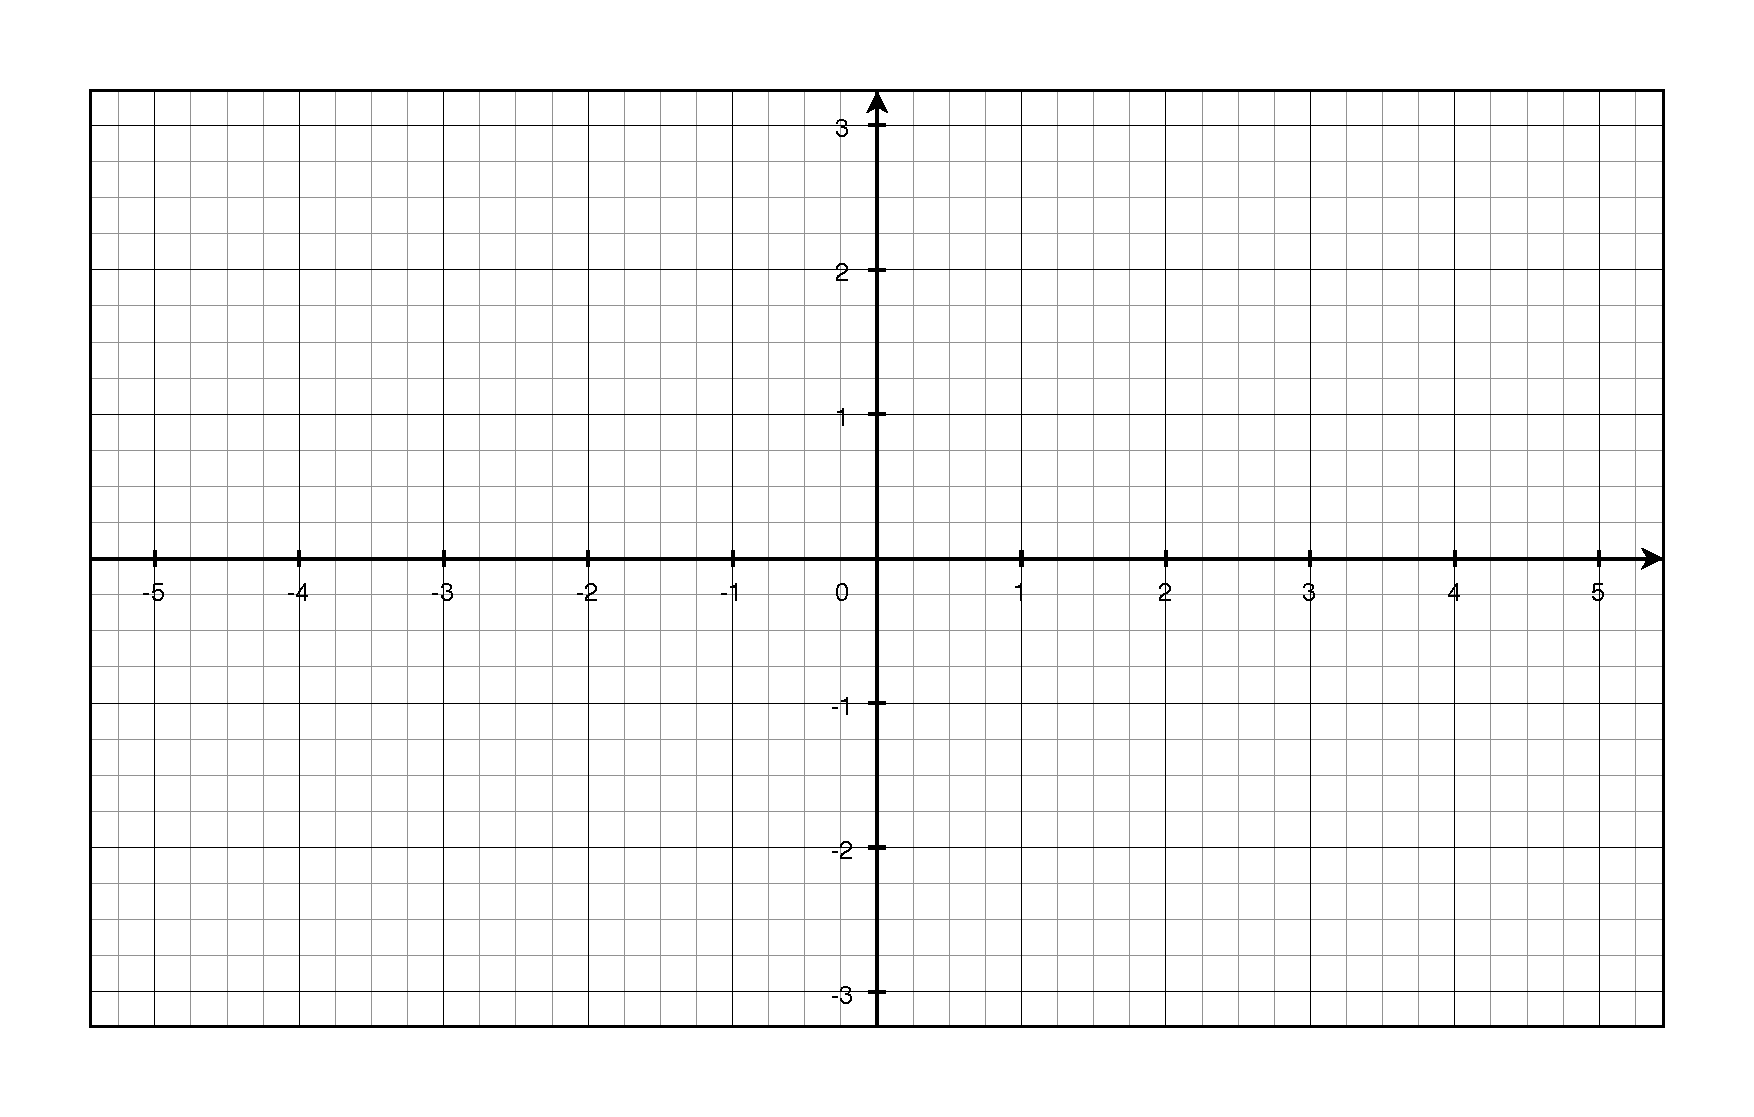
\includegraphics[scale=0.6]{graph_2_blank.eps}
  \caption*{Question \ref{graph:2}}
\end{figure}
\fi

\ifprintanswers
\else
\pagebreak
\fi

\question[15]
\label{graph:3}

\[
  f(x) = \frac{x^2+x-2}{x+3} 
\]

\begin{solution}[6 cm]

\[
  f(x) = \frac{x^2+x-2}{x+3} = \frac{(x+2)(x-1)}{x+3}
\]

\begin{itemize}
  \item since the degree of the numerator is one more than the degree of the denominator, there is a slant asymptote.
    Long division shows the asymptote is at $y = x-2$.

  \item there is a vertical asymptote at $x=-3$
  \item the x intercepts are at: $x = \{ -2, 1 \}$ 
  \item $f(0) = -\dfrac{2}{3}$, so the y intercept is at $y = -\dfrac{2}{3}$
\end{itemize}

\end{solution}

\ifprintanswers
\begin{figure}[H]
  \centering
  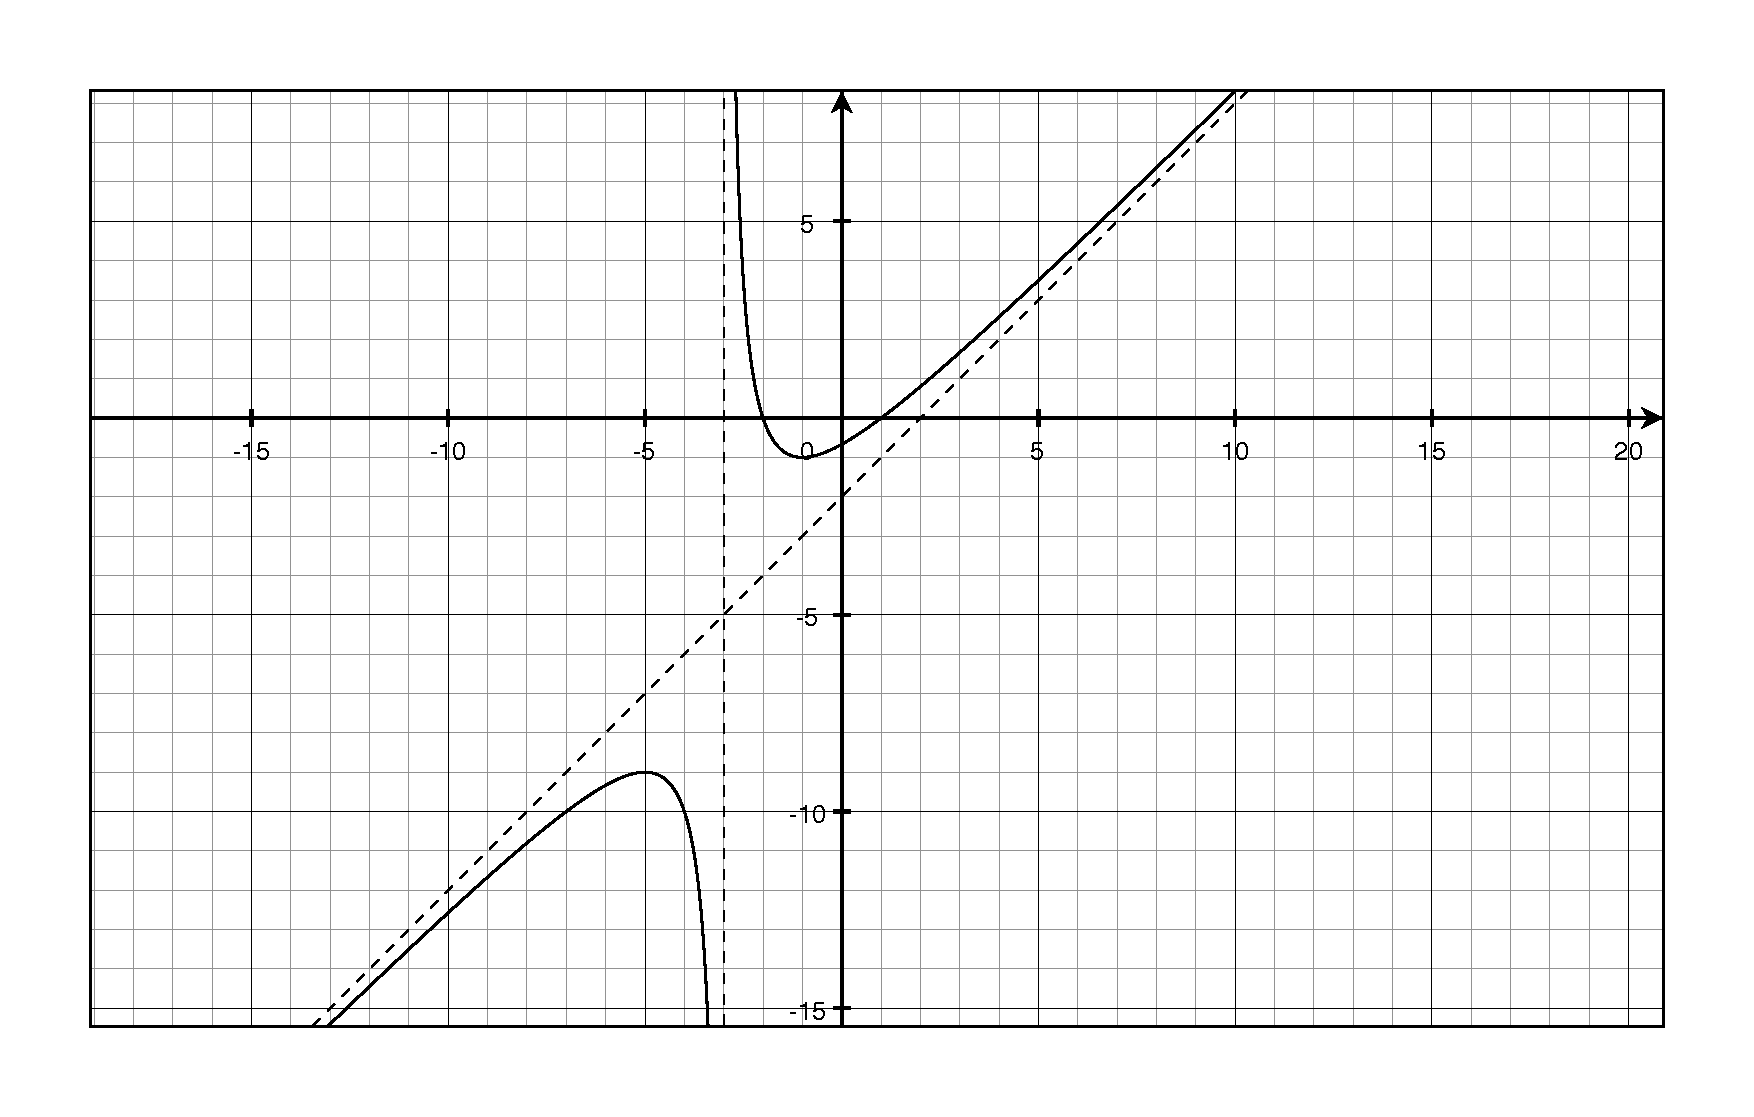
\includegraphics[scale=0.4]{graph_3_solution.eps}
  \caption*{Question \ref{graph:3}}
\end{figure}
\else
\begin{figure}[H]
  \centering
  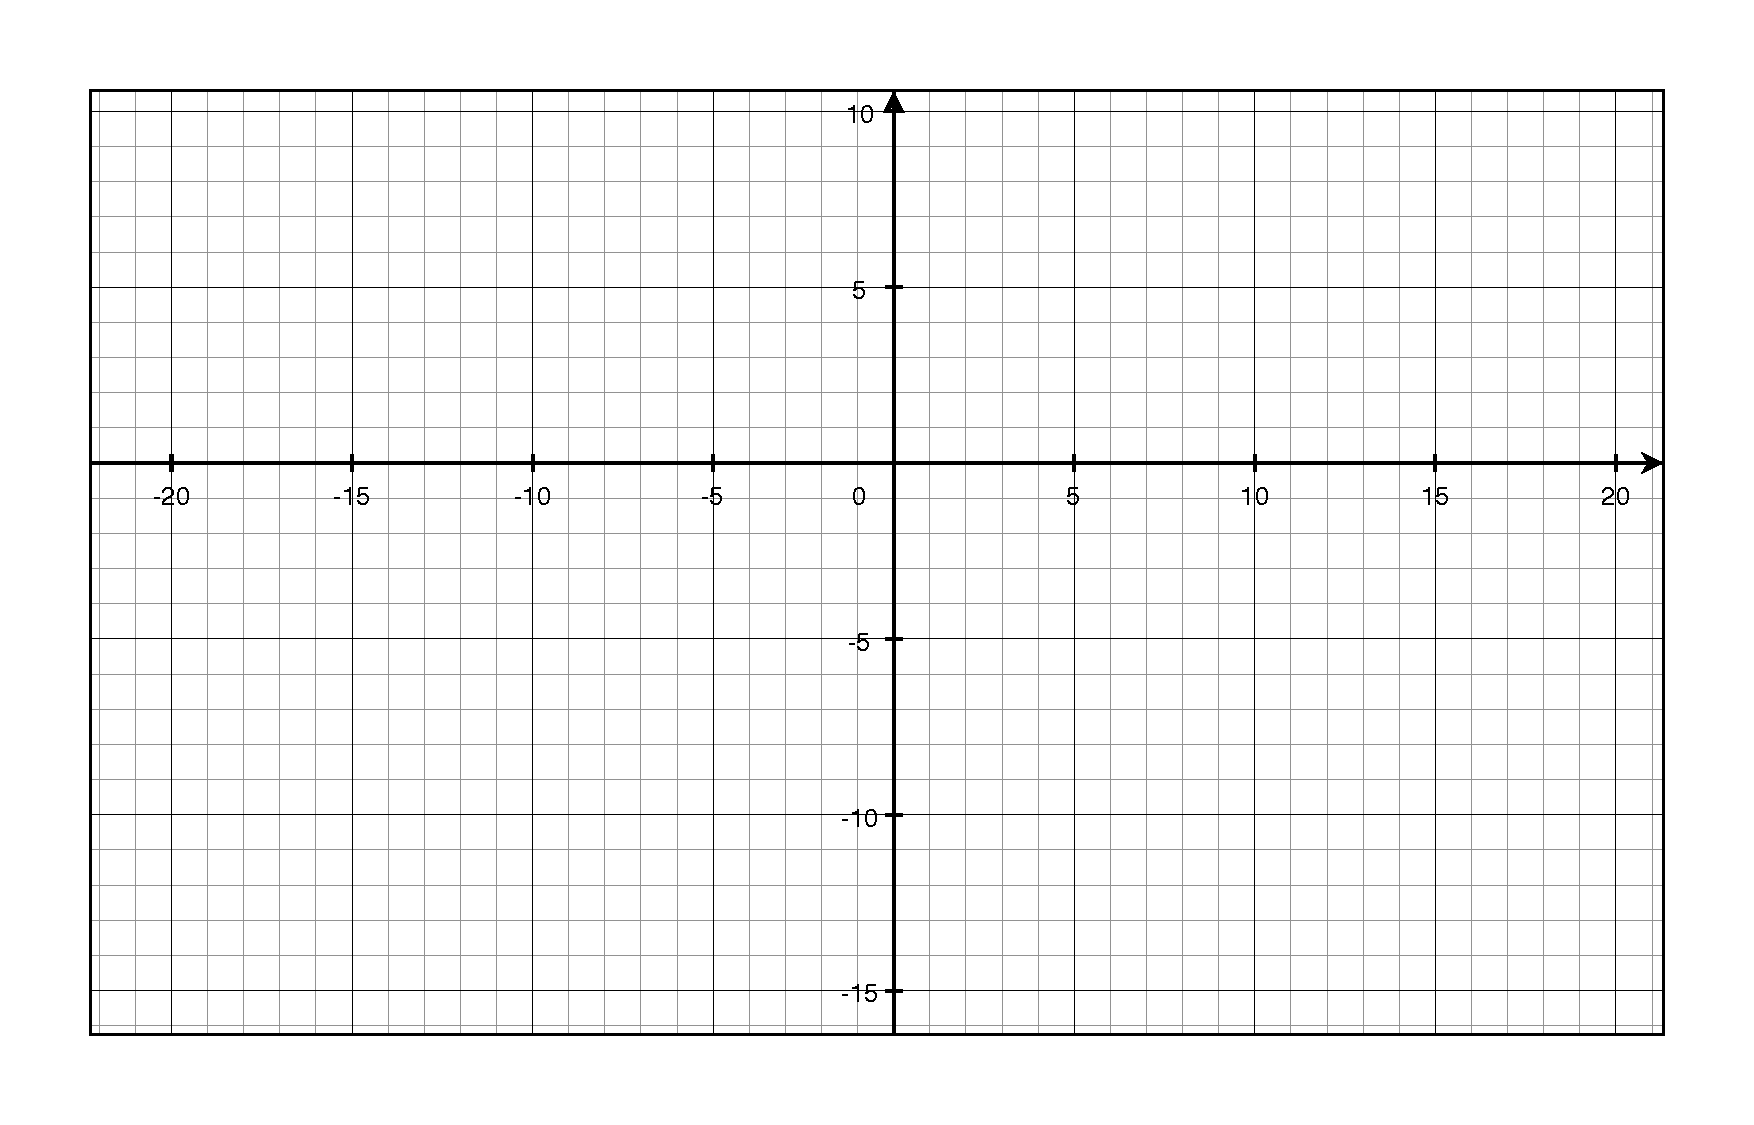
\includegraphics[scale=0.6]{graph_3_blank.eps}
  \caption*{Question \ref{graph:3}}
\end{figure}
\fi

\pagebreak

\section{Extra Credit}
\bonusquestion[10]

Remember that if $z$ is a complex number, $\overline{z}$ is the conjugate of $z$.

If $x$ and $y$ are complex numbers and $a$ is a real number:
\begin{itemize}
  \item $\overline{x} \cdot \overline{y} = \overline{x \cdot y}$
  \item $\overline{x} + \overline{y} = \overline{x + y}$
  \item $\overline{a} = a$
\end{itemize}

Use these rules to show that if
\[
  f(x) = a_3 x^3 + a_2 x^2 + a_1 x + a_0
\]
and $f(z) = 0$ then $f(\overline{z}) = 0$

\begin{solution}[2 cm]
\begin{align*}
  f(\overline{z}) &= a_3\overline{z}^3 + a_2\overline{z}^2 + a_1\overline{z} + a_0 & \\
     &= \overline{a_3 z^3} + \overline{a_2 z^3} + \overline{a_1 z} + a_0           & \text{(rules 1 and 3)} \\
     &= \overline{a_3z^3 + a_2z^2 + a_1z} + a_0                                    & \text{(rule 2)} \\
     &= \overline{a_3z^3 + a_2z^2 + a_1z} + \overline{a_0}                         & \text{(rule 3)} \\
     &= \overline{a_3z^3 + a_2z^2 + a_1z + a_0}                                    & \text{(rule 2)} \\
     &= \overline{f(z)}                                                           & \text{(definition of f)} \\
     &= \overline{0}                                                              & (f(z) = 0) \\
     &= 0                                                                         & \text{(rule 3)} \\
\end{align*}

\end{solution}

\end{questions}

\end{document}
